% To compile single chapters put a % symbol in front of "\comment" and "}%end of comment" below 
%    and take off the % symbol from "\end{document" at the bottom line. Undo before compiling
%    the complete thesis
%%Note: You can only use \section command, you are not allowed, per TTU Graduate School, use
%%\subsection command for ghigher level subheadings. At most level 2 subheadings are allowed.

\chapter{DASP Image Processing and Feature Extraction}
\label{DASP Feature Extraction Chapter}

\section[DASP Image Pre-Processing]{DASP Image Pre-Processing}
\label{DASP Image Pre-Processing Section}

The suite of DASP algorithms presented in Chapter \ref{DASP Algorithm Development Chapter} provide methods for aligning and highlighting signal dimensions, such as modulations and harmonics, that are inherent to URE conducted from electronic equipment.  The resulting alignments can take a variety of shapes within the DASP images, from straight lines to curved lines to crossing radials to signal peaks; however, direct feature extraction from the raw DASP images can be problematic because of scaling, dynamic range, and confounding signal structures.

Multiple image processing and feature extraction techniques were utilized to prepare the DASP images for machine learning analysis.  Two machine learning techniques were explored, a feature vector based approach and an image classification learning method, with both requiring different DASP image pre-processing methods.  Both learning methods required the DASP images to be scaled to limit dynamic range and remove the background noise, as outlined in Section \ref{Image Scaling}.  To further highlight features of interest, such as lines and peaks, the raw DASP images were also processed with thresholding, edge, and line detection algorithms, as described in Sections \ref{Threshold Processing} and \ref{Edge and Line Detection}.  The image classification technique operated directly on the scaled and processed images with no further feature extraction required, whereas the DASP images were further processed through an image segmentation, matrix summing, and statistical measurement process to form feature vectors for the feature vector machine learning algorithms, as outlined in Sections \ref{Image Segmentation} and \ref{Statistical Feature Extraction}.

\subsection[Image Scaling]{Image Scaling}
\label{Image Scaling}

DASP images can suffer from dynamic range issues resulting from the large differences ($10$s of dB) in measured URE signal levels from a single device or across multiple devices, which can further be exacerbated by the bit growth associated with the continual multiplication and summing steps that comprise the DASP processes.  In addition, different parts of a given URE spectrum can vary widely because of broadband noise or narrowband frequency peaks unrelated to the device under test.  To normalize and scale DASP images before further image processing or feature extraction the image scaling algorithm described in Algorithm \ref{alg:imscalealg} was initially applied to all DASP generated images. 

\begin{algorithm}
	\caption{Image Scaling Algorithm} \label{alg:imscalealg}
	\scriptsize
	\begin{algorithmic}[1]
		\Require~~
		\Statex $\mathbf{I}$ - Input Image
		\Statex $\mathbf{I_b}$ - Background Image
		\Ensure~~
		\Statex $\mathbf{I_s}$ - Scaled Image Output
		\Statex
		\State $\mathbf{I_s} \gets \mathbf{I} - \mathbf{I_b}$ 
		\State $\mathbf{I_s} \leq 0 \gets 0$
		\State $\mathbf{I_s}  \gets $ STANDARD DEVIATION FILTER of $\mathbf{I_s}$
		\State $\mathbf{I_s} = \log{\mathbf{I_s}}$
	\end{algorithmic}
\end{algorithm}

The URE collection process outlined in Chapter \ref{URE Data Collection Chapter} recorded $24000$ \textit{off} state captures of which $22800$ were randomly selected and removed from the test and training data set to generate a representative background for DASP device image normalization.  The removal of the extra \textit{None} state captures also balanced the number of samples per class and eliminated any concerns regarding class skew in the learning process.  The $22800$ \textit{off} state DASP images were averaged together to form a background image, $\bf{I_b}$, which was subtracted from the raw DASP images, $\bf{I}$, to generate a scaled image, $\bf{I_s}$.   A rectifying linear transformation was then applied to $\bf{I_s}$ followed by a standard deviation image filter resulting in a localized z-score across the entire image.  Finally, a logarithm was applied to each pixel of entire image to further reduce the dynamic range of the scaled image.  

\subsection[Threshold Processing]{Threshold Processing}
\label{Threshold Processing}

The MASP algorithm was specifically developed to generate a peak at the intersection of a modulation frequency and carrier frequency.  These peaks are often obscured within the MASP image because of a large dynamic range or by being masked by unmodulated portions of a carrier frequency, as can be seen in Figure \ref{fig:masp_example}.  To highlight peaks within a MASP image a threshold processing algorithm was developed to generate a scatter plot with each scatter point representing a detected peak in the original image.  The algorithm is described in Algorithm \ref{alg:scatteralg} and operates on an input MASP image, $\mathbf{I}$, with the fill ratio, $p$, input parameter which determines the total number of scatter points to generate in the final scatter plot.   

\begin{algorithm}
	\caption{Scatter Plot Peak Detection Algorithm} \label{alg:scatteralg}
	\scriptsize
	\begin{algorithmic}[1]
		\Require~~
		\Statex $\mathbf{I}$ - Input Image
		\Statex $p$ - Fill Ratio
		\Ensure~~
		\Statex $\mathbf{S}$ - Detected Scatter Points
		\Statex
		\Statex Initialize THRESHOLD 
		\While {$1.1p < $ fill $ < 0.9p$}
			\State $\bf{I_t} \gets $ ZSCORE for each row of $\bf{I}$
			\State $\bf{I_t} \gets 0$ for all $\bf{I_t} \le$ THRESHOLD
			\State $\bf{I_t} \gets $ ZSCORE for each column of $\bf{I_t}$ for all $\bf{I_t} \ne 0$
			\State INITIALIZE $\bf{S} = 0$
			\For {elements of $\bf{I_t} \geq $ THRESHOLD}
				\State $\mathbf{S} \gets 1$
			\EndFor
			\State fill $ \gets \sum{\bf{S}}$
			\State UPDATE THRESHOLD
		\EndWhile
	\end{algorithmic}
\end{algorithm}

The scatter plot algorithm initializes a threshold which is iterated on until the number of scatter points is within $10\%$ of the fill ratio.  The algorithm separately scales and thresholds the rows and columns of an image to only generate scatter points that exceed a given threshold in both directions.  After thresholding, the total number of scatter points is calculated and the threshold value is updated to either increase or decrease the number of scatter points based upon the difference between the fill ratio and the total number of scatter points in the current iteration.

To illustrate the scatter point threshold algorithm and image output, the scatter plot peak detection algorithm was applied to the MASP image in Figure \ref{fig:masp_example} and is shown in Figure \ref{fig:maspl_scatter}.  The scatter plot shows groupings, rows, and columns of scatter points that identify modulation peaks that were not easily identifiable in the original MASP image.  For instance, the row of points at $f_m = 26$Hz indicate a significant number of higher frequency carriers being modulated by $26$Hz, which is not obvious in the original MASP image in Figure \ref{fig:masp_example}.

\begin{figure}[tb]
	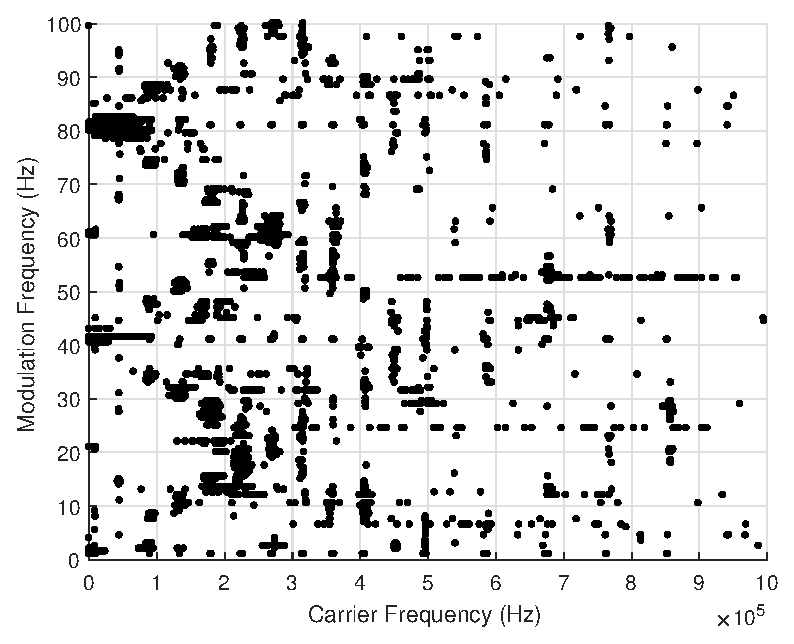
\includegraphics[width=\textwidth]{./dasp_algorithm_results/masp_low_scatter_filenum_12001.eps}
	\centering
	\caption{Scatter plot resulting from the peak thresholding of the MASP image in Figure \ref{fig:masp_example}.  The scatter plot highlights peaks in the MASP image that would otherwise not be visible due to dynamic range of the image, such as the row of points located at the $26$Hz modulation frequency.  It should also be noted that the horizontal lines at $20$Hz and $60$Hz in Figure \ref{fig:masp_example} are no longer visible because their magnitudes did not exceed the threshold in both the vertical and horizontal dimensions.}
	\label{fig:maspl_scatter}
\end{figure}

In addition to the row of modulations at $26$Hz, its second harmonic at $52$Hz also showed a similar broadband modulation pattern.  Several modulation structures became evident upon further examination, such as the large clustering of modulations at the intersection of $80$Hz with low frequency carriers and the large number of clusters between the $100$kHz and $200$kHz carrier frequencies.  By performing the scatter point thresholding against the rows and columns of the MASP image, the resulting scatter plot can highlight modulation structures that are not evident in the raw images.   

\subsection[Edge and Line Detection]{Edge and Line Detection}
\label{Edge and Line Detection}

Several of the DASP algorithms result in images that contain dimensional alignments that generate straight and curved lines, such as with HASP and CMASP, and much like the scatter plot peak detection algorithm for the MASP images, tailored transforms were required to highlight and exploit these features.  To highlight lines and edges within a DASP image a Laplacian of Gaussian (LoG) edge detector \cite{Marr1980} was applied to the DASP images using the MATLAB\textsuperscript \textregistered ~ \textit{edge} function\footnote{https://www.mathworks.com/help/images/ref/edge.html, June $26$, $2017$}.  Figure \ref{fig:cmasp_edge} shows the resulting image after application of the LoG edge detector to the image in Figure \ref{fig:cmasp_example} while using a LoG filter standard deviation value of $2$ and a filter size of $13 \times 13$.  

\begin{figure}[tb]
	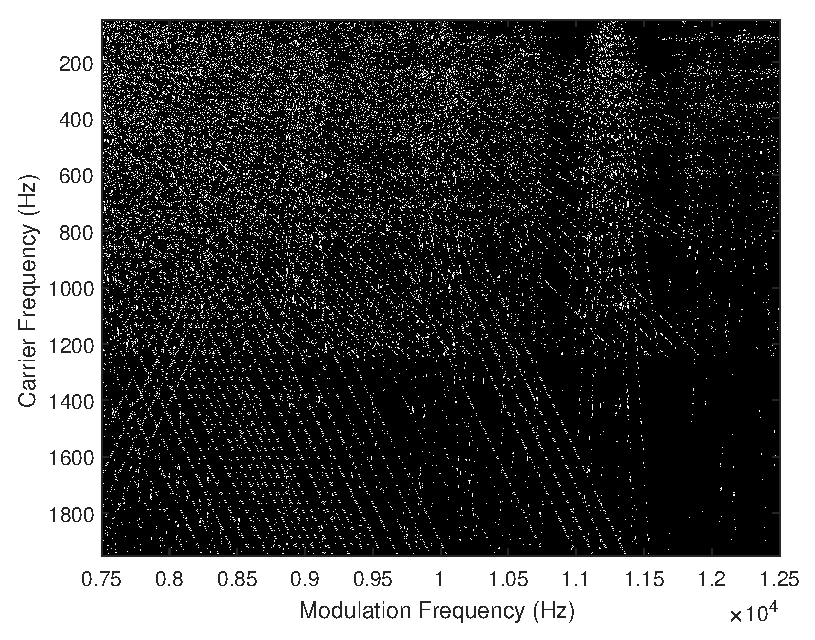
\includegraphics[width=\textwidth]{./dasp_algorithm_results/cmasp_edge_filenum_9601.eps}
	\centering
	\caption{CMASP image resulting from the application of a LoG edge detector to the image in Figure \ref{fig:cmasp_example}.  The edge detection algorithm removes variations in the background and highlights edges and lines for subsequent feature extraction or line detection processing.}
	\label{fig:cmasp_edge}
\end{figure}

Application of the LoG edge detector highlighted discontinuities in the processed image, resulting in an image with detection points forming lines and other shapes outlining the structures within the original image.  A radon transform \cite{Deans1981} was then applied to the CMASP edge detection image, Figure \ref{fig:cmasp_edge}, to detect radial lines traversing the image, as shown in Figure \ref{fig:cmasp_radon}.  The MATLAB\textsuperscript \textregistered ~ \textit{radon} function \footnote{https://www.mathworks.com/help/images/ref/radon.html, June $26$, $2017$} was utilized with projection angles between $0^{\circ}$ and $180^{\circ}$.  Figure \ref{fig:cmasp_radon} shows the radon output image along with detected peaks highlighted with circles, while Figure \ref{fig:cmasp_peak} provides a mesh plot of the same image to better illustrate image peaks.  Each peak in the radon image corresponds to a detected line at a given location ($x'$) and angle.
  
\begin{figure}[tb]
	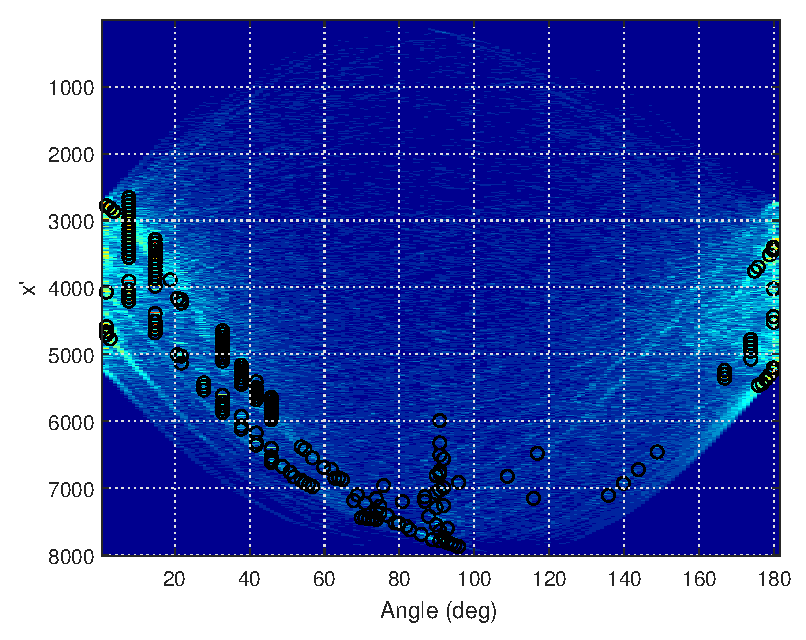
\includegraphics[width=\textwidth]{./dasp_algorithm_results/cmasp_radon_filenum_9601.eps}
	\centering
	\caption{Radon transform of the CMASP image in Figure \ref{fig:cmasp_edge} with detected peaks highlighted with circles.  Each detected peak corresponds to a line in the original image.  The vertically aligned circles in the center of the image correspond to vertical lines in the original image and the circles in the left and right quadrants correspond to angled lines in the original image with the x-axis providing the angle and the y-axis the location.}
	\label{fig:cmasp_radon}
\end{figure}

\begin{figure}[tb]
	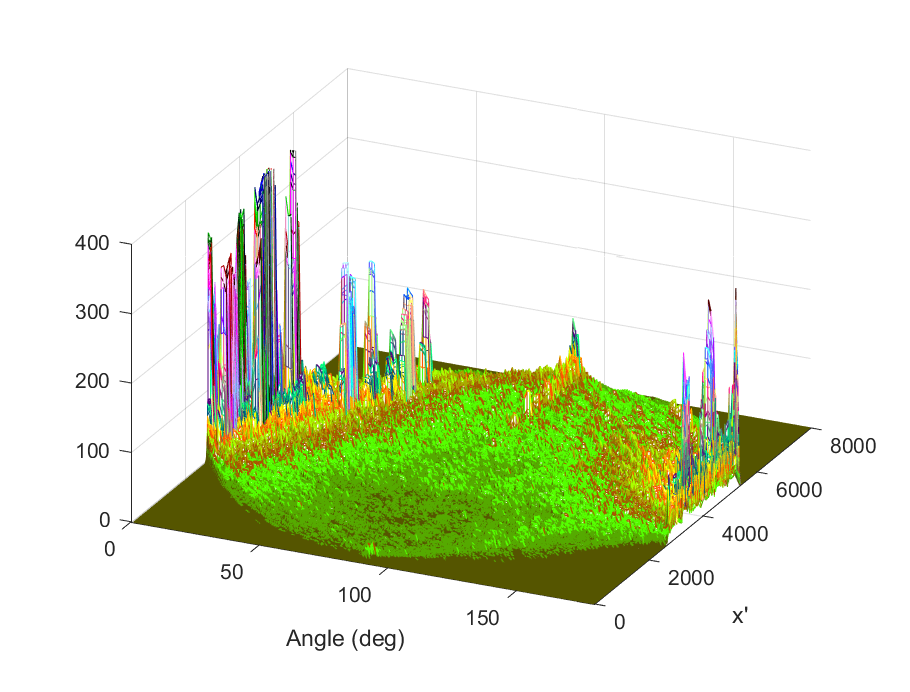
\includegraphics[width=\textwidth]{./dasp_algorithm_results/cmasp_radon_mesh_filenum_9601.eps}
	\centering
	\caption{Mesh plot of the radon transformed CMASP image in Figure \ref{fig:cmasp_edge} illustrating the detected peaks.}
	\label{fig:cmasp_peak}
\end{figure}

The LoG and radon functions provide a suite of tools for highlighting lines and edges within a DASP image.  As can be seen in Figure \ref{fig:cmasp_example}, the CMASP transform can generate many lines with no clear structure which could potentially confound and mask underlying discriminative features.  The application of the LoG edge detector can eliminate much of the underlying noise and highlight lines and edges of interest, while the subsequent application of the radon transform can detect highlighted lines and potentially provide a more compact representation of the CMASP image structure.  For instance, the large number of detected peaks in Figure \ref{fig:cmasp_radon} provided indications of a large number of distinct and left-to-right downward sloping lines, as evident in Figure \ref{fig:cmasp_edge}.

\subsection[Images Segmentation]{Image Segmentation}
\label{Image Segmentation}

Dimensional alignments or other features of interest relevant for the classification of URE generators occur within different regions of the DASP images.  To aid in feature extraction and to isolate features of interest, an image segmentation process was developed to generate sub-segments of an input DASP image.  The image segments are illustrated in Figure \ref{fig:haspd_segment}.  The segmentation of Figure \ref{fig:haspd_example} shows the isolation of aligned harmonics in segments $8$, $5$, and $2$.  In addition, the process also generated segments which did not contain features of interest for this particular device; however, other devices may generate features that do occur in these segments and therefore provide better discrimination for the purposes of classification. 

\begin{figure}[tb]
	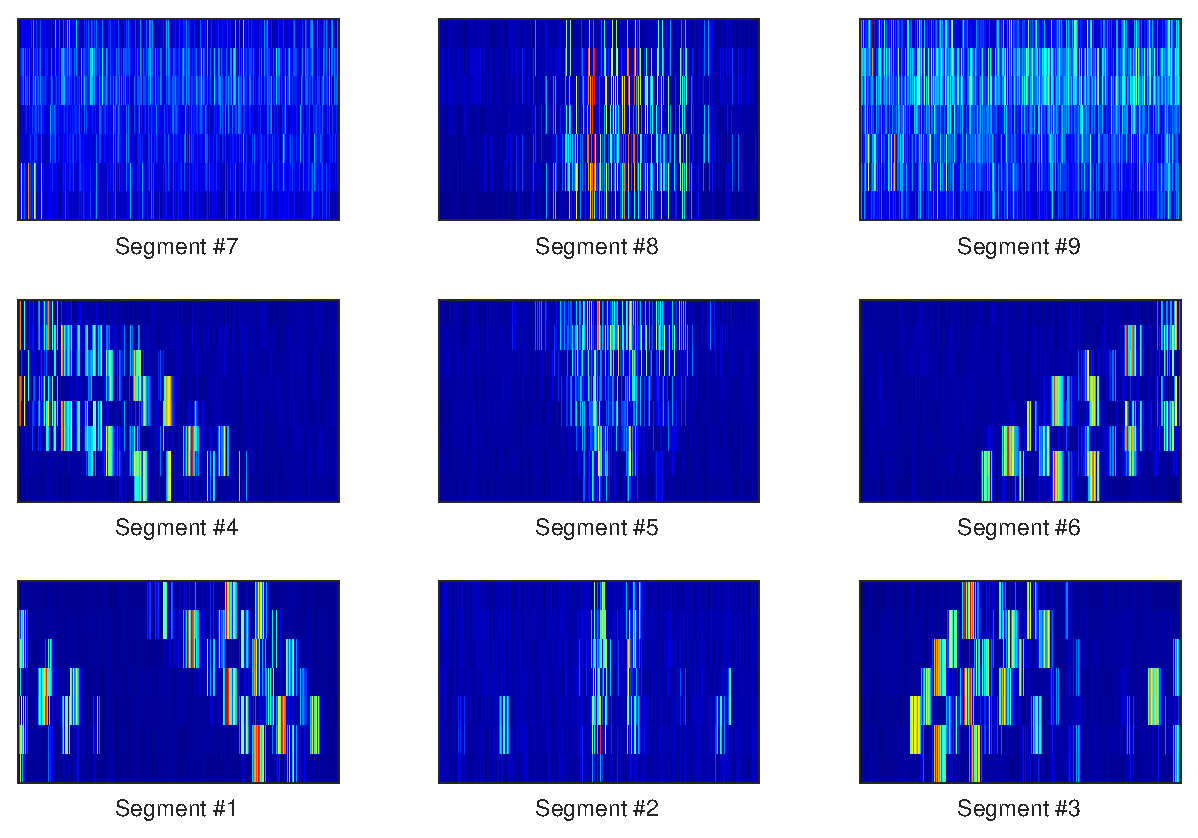
\includegraphics[width=\textwidth]{./dasp_algorithm_results/hasp_segment_filenum_12001.eps}
	\centering
	\caption{$3 \times 3$ image segmentation of the image in Figure \ref{fig:haspd_example} demonstrating the isolation of specific regions of interest.  By segmenting the image, features of interest can further be highlighted without confounders, such as in the center-bottom tile, segment $\#2$.}
	\label{fig:haspd_segment}
\end{figure}

\section[Statistical Feature Extraction]{Statistical Feature Extraction}
\label{Statistical Feature Extraction}

Extraction of features from the DASP images can be tailored to a specific device or class given \emph{a priori} knowledge of the URE characteristics, such as specific frequency peaks or modulation frequencies.  Given no prior knowledge of a device's URE characteristics and the low noise collection environment, no tailored feature extractors were utilized in the feature generation process.  Two machine learning classification techniques are explored in Chapter \ref{DASP Device Classification Chapter}. The first machine learning approach was based upon 1-D statistical feature vectors extracted from DASP images, while the second machine learning technique used was the CNN deep learning approach applied directly to the DASP images.   

General statistical features based on variance ($\sigma^2$), skewness ($\gamma$), and kurtosis ($\kappa$), as defined by Equations \ref{eq:sigmaeq}, \ref{eq:gammaeq}, and \ref{eq:kappaeq}, respectively, were extracted from the DASP images to form a 1-D feature vector for machine learning, as also demonstrated by \cite{Zhenfei2009}, \cite{Klein2009}, \cite{Lukacs2016}, and \cite{Cobb2010}.  Samples over which to compute the statistics were taken from the summed rows and columns of each image, or image segment, as illustrated in Figure \ref{fig:haspd_summation}.  For whole image feature extraction, all of the pixels of the image were concatenated into a single vector and used as samples for statistical feature generation.  

\begin{equation}
	\sigma^{2}_{\bf{x}} = \textbf{E}[(\textbf{x} - \mu)^2]
	\label{eq:sigmaeq}
\end{equation}

\begin{equation}
	\gamma_{\bf{x}} = \textbf{E}\left[\left(\frac{\textbf{x} - \mu}{\sigma}\right)^3\right]
	\label{eq:gammaeq}
\end{equation}

\begin{equation}
	\kappa_{\bf{x}} = \frac{\textbf{E}[(\textbf{x} - \mu)^4]}{(\textbf{E}[(\textbf{x} - \mu)^2])^2}
	\label{eq:kappaeq}
\end{equation}

where $\bf{x}$ are the samples taken from the summed rows, summed columns, and concatenated pixel vector of the DASP arrays shown in Figure \ref{fig:haspd_summation}.

\begin{figure}[ht]
	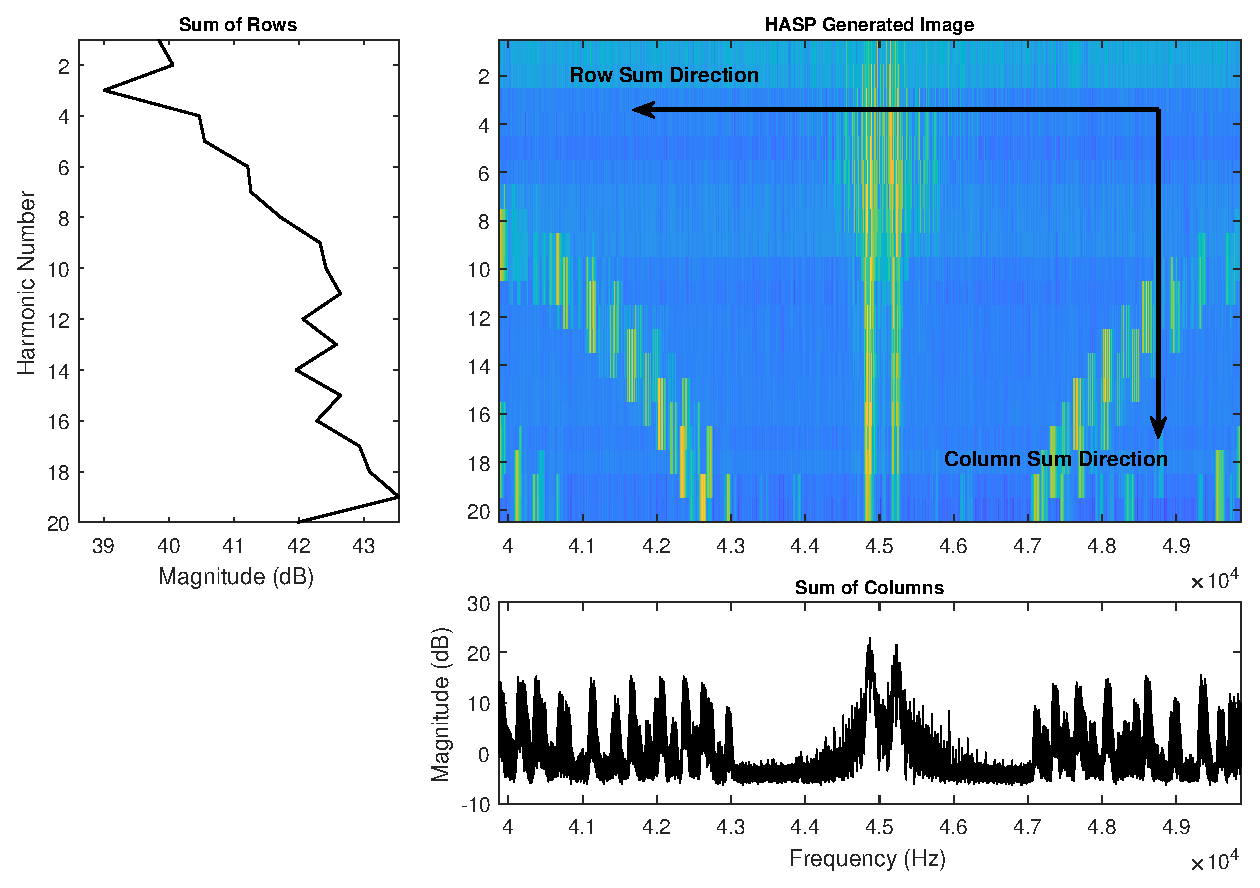
\includegraphics[width=\textwidth]{./dasp_algorithm_results/hasp_d_summing_filenum_9601.eps}
	\centering
	\caption{Column and row summing as applied to the HASP-D image shown in Figure \ref{fig:haspd_example}.  By aligning the independent carriers and their respective harmonics in the HASP-D image, the column summing provides a method for adding the ``coherent'' energy associated with the independent carriers, providing a significant response in the resulting summed vector.}
	\label{fig:haspd_summation}
\end{figure}

As illustrated in Figure \ref{fig:haspd_summation}, the HASP-D algorithm aligns harmonically related frequencies into a single column within the HASP-D image and the column summing allows all of the related harmonics to be added coherently into a single vector as demonstrated in the sum of columns plot.   Although not as pronounced in Figure \ref{fig:haspd_summation}, the row summing can provide insights into the harmonic structure of the underlying signal.  For instance, the summed row vector shows an alternating harmonic intensity structure between the $11$th and $17$th harmonics.

%\section[Image Structural Similarity]{Image Structural Similarity}
%
%\blindtext[1]
%
%\begin{equation}
	%SSIM(x,y) = \left[i(x,y)\right]^{\alpha}\left[c(x,y)\right]^{\beta}\left[S(x,y)\right]^{\gamma} 
	%\label{eq:ssimeq}
%\end{equation}
%
%where
%
%\begin{equation}
	%i(x,y) = \left[i(x,y)\right]^{\alpha}\left[c(x,y)\right]^{\beta}\left[s(x,y)\right]^{\gamma} 
	%\label{eq:ssimieq}
%\end{equation}
%
%\begin{equation}
	%c(x,y) = \frac{2\mu_{x}\mu_{y} + C_{1}}{\sigma^{2}_{x} +\sigma^{2}_{y} + C_{2}}
	%\label{eq:ssimceq}
%\end{equation}
%
%\begin{equation}
	%s(x,y) = \left[i(x,y)\right]^{\alpha}\left[c(x,y)\right]^{\beta}\left[S(x,y)\right]^{\gamma} 
	%\label{eq:ssimseq}
%\end{equation}
%
%\begin{figure}[ht]
	%\includegraphics[width=\textwidth]{./dasp_algorithm_results/masp_refimage_ssim_device_6.eps}
	%\centering
	%\caption{Reference MASP image generated by averaging $20$ MASP images derived from URE collected from fluorescent lights and subtracting the background (i.e. the ``None'' state).}
	%\label{fig:masp_ref_image}
%\end{figure}
%
%\begin{figure}[ht]
	%\includegraphics[width=\textwidth]{./dasp_algorithm_results/masp_image_ssim_refcmp_device_6.eps}
	%\centering
	%\caption{Plot of structural similarity index values between MASP reference image of device $6$ and a random sampling of MASP images from all $20$ devices.  The peak at $6$ shows the highest similarity to device $6$, which confirms the applicability of comparing DASP images through SSIM values.}
	%\label{fig:masp_ssim_dev}
%\end{figure}
%
%\begin{figure}[ht]
	%\includegraphics[width=\textwidth]{./dasp_algorithm_results/masp_image_ssim_multrefcmp_device_6.eps}
	%\centering
	%\caption{Image of SSIM values using a comparison of the MASP reference image for device $6$ to captures with all combinations of two devices present.  The peaks at the rows and columns at $6$ show that even with confounders the SSIM still shows a peak when device $6$ is present and further shows that the SSIM to all other combinations of devices is low.}
	%\label{fig:masp_ssim_multi}
%\end{figure}



%\begin{figure}[ht]
	%\includegraphics[width=\textwidth]{./dasp_algorithm_results/masp_summing_filenum_9601.eps}
	%\centering
	%\caption{Column and row summing as applied to the MASP image shown in \ref{fig:masp_example}.  The row summing highlights the relative strengths and location of the modulating frequencies.}
	%\label{fig:masp_summation}
%\end{figure}

%\subsubsection[Clustering Analysis]{Cluster Analysis}
%
%\blindtext[1]
%
%\begin{figure}[ht]
	%\includegraphics[width=\textwidth]{./dasp_algorithm_results/masp_dbscan_noise_filenum_12001.eps}
	%\centering
	%\caption{MASP Scatter DBSCAN with Noise}
	%\label{fig:maspdbscannoise}
%\end{figure}
%
%\begin{figure}[ht]
	%\includegraphics[width=\textwidth]{./dasp_algorithm_results/masp_dbscan_nonoise_filenum_12001.eps}
	%\centering
	%\caption{MASP Scatter DBSCAN without Noise}
	%\label{fig:maspdbscanwithoutnoise}
%\end{figure}
%
%\begin{figure}[ht]
	%\includegraphics[width=\textwidth]{./dasp_algorithm_results/masp_blob_area_filenum_12001.eps}
	%\centering
	%\caption{MASP Blob analysis with detected corners}
	%\label{fig:maspblob}
%\end{figure}
%
%\begin{figure}[ht]
	%\includegraphics[width=\textwidth]{./dasp_algorithm_results/hasp_dbscan_nonoise_filenum_12001.eps}
	%\centering
	%\caption{HASP Scatter DBSCAN without Noise}
	%\label{fig:haspdbscanwithoutnoise}
%\end{figure}
%
%\begin{figure}[ht]
	%\includegraphics[width=\textwidth]{./dasp_algorithm_results/hasp_blob_area_filenum_12001.eps}
	%\centering
	%\caption{HASP Blob analysis with detected corners}
	%\label{fig:haspblob}
%\end{figure}
%\subsection[Histogram Based Features]{Histogram Based Features}
%
%\begin{figure}[ht]
	%\includegraphics[width=\textwidth]{./dasp_algorithm_results/masp_hist_filenum_12001.eps}
	%\centering
	%\caption{MASP Aligned Histogram}
	%\label{fig:masphist}
%\end{figure}
%
%\begin{figure}[ht]
	%\includegraphics[width=\textwidth]{./dasp_algorithm_results/masp_segment_filenum_12001.eps}
	%\centering
	%\caption{$3 \times 3$ image segmentation of the \ref{fig:masp_summation} image isolating specific regions of interest.  Tiling of the MASP image highlights specific locations of peaks associated with the intersection of carrier and modulation frequencies, such as illustrated in the top two rows of tiles.} 
	%\label{fig:masp_segment}
%\end{figure}


